\chapter{Additional figures}


% \section{Validation of error bounds}\label{app:extra_paper_plots}


% \begin{figure}
% 	\begin{center}
% 		\begin{subfigure}{\textwidth}
% 			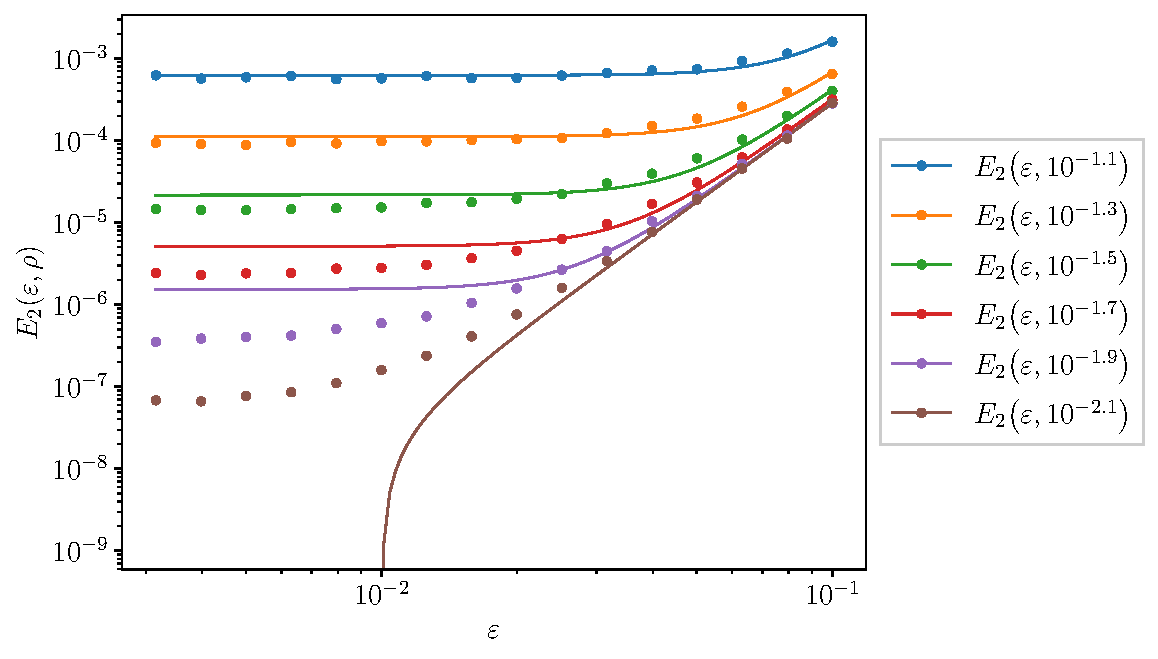
\includegraphics[width=0.49\textwidth]{chp04_paper_numerics/figures/sine/str_err_eps_r_2.0_log.pdf}
% 			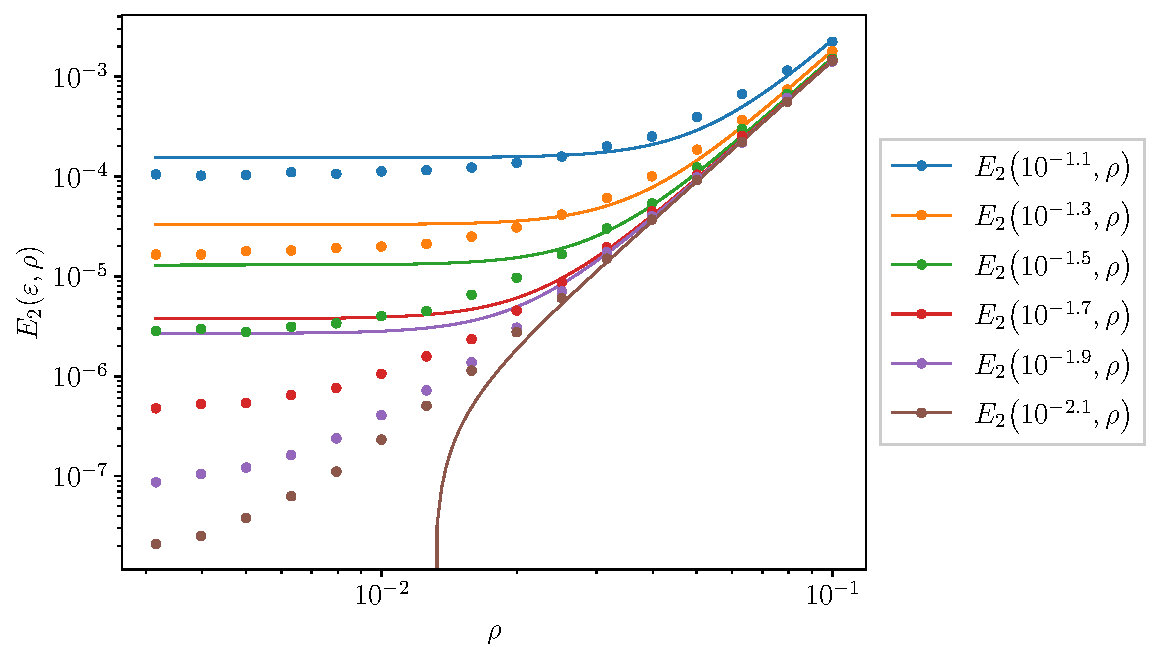
\includegraphics[width=0.49\textwidth]{chp04_paper_numerics/figures/sine/str_err_rho_r_2.0_log.pdf}
% 			\caption{\(r = 2\)}
% 		\end{subfigure}
% 		\begin{subfigure}{\textwidth}
% 			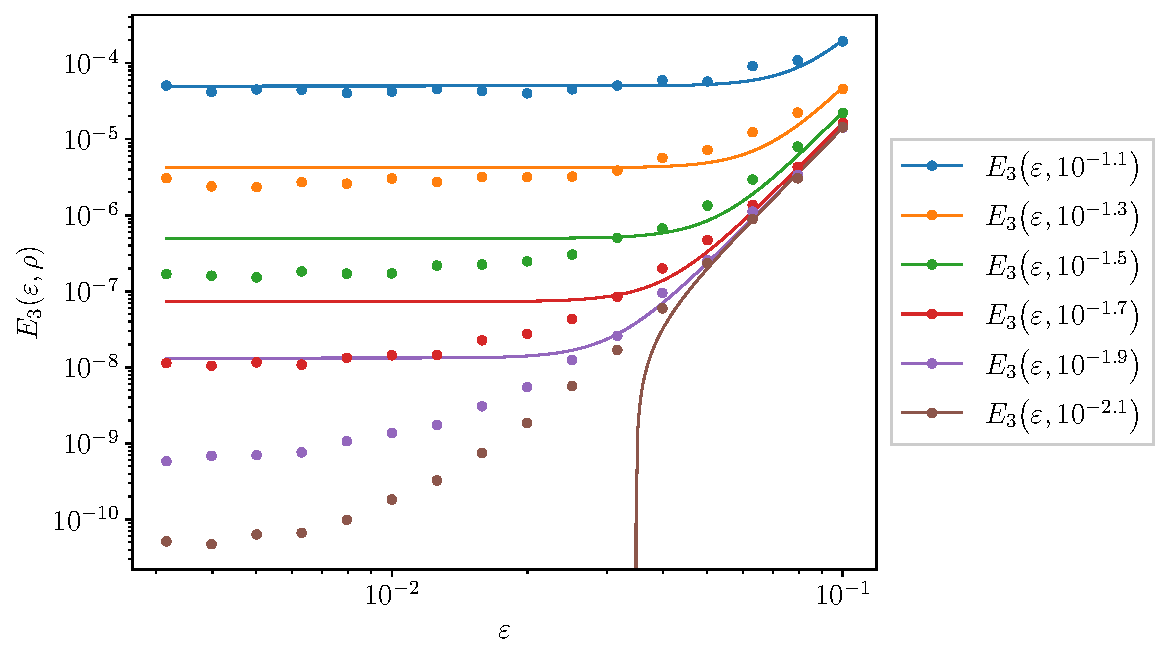
\includegraphics[width=0.49\textwidth]{chp04_paper_numerics/figures/sine/str_err_eps_r_3.0_log.pdf}
% 			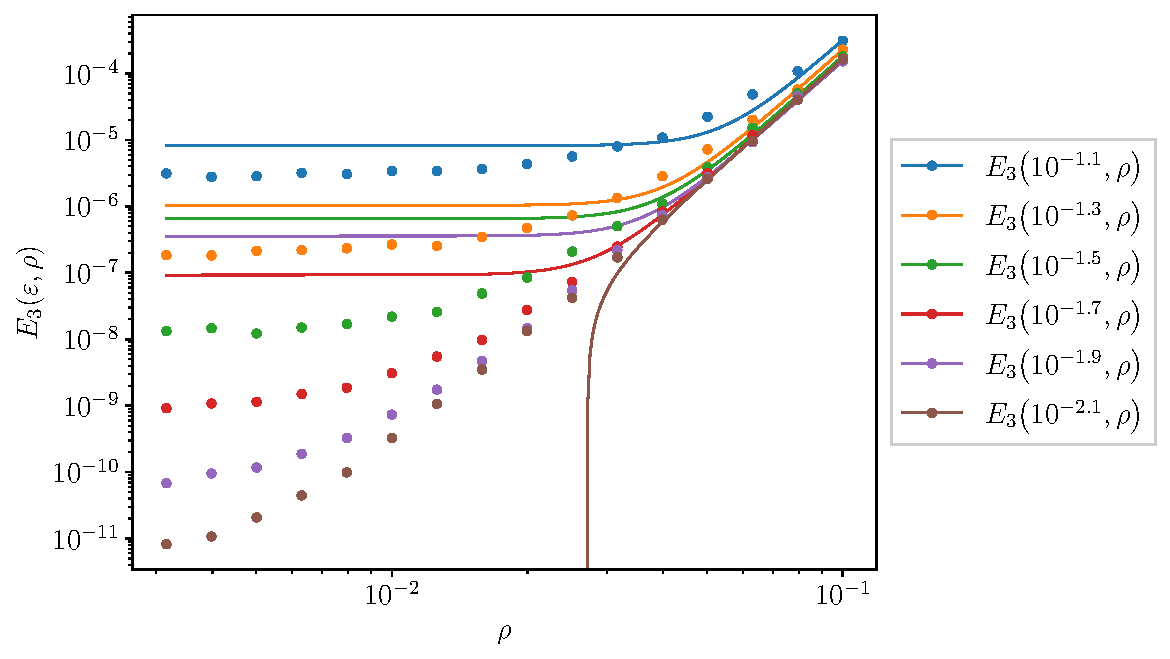
\includegraphics[width=0.49\textwidth]{chp04_paper_numerics/figures/sine/str_err_rho_r_3.0_log.pdf}
% 			\caption{\(r = 3\)}
% 		\end{subfigure}
% 		\begin{subfigure}{\textwidth}
% 			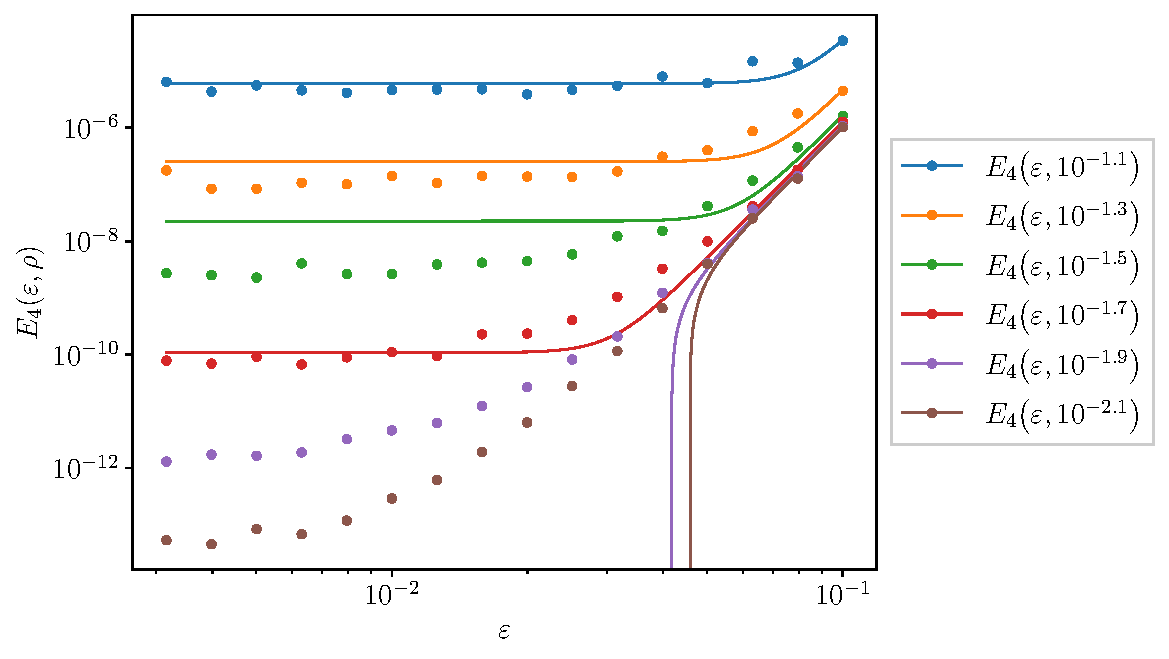
\includegraphics[width=0.49\textwidth]{chp04_paper_numerics/figures/sine/str_err_eps_r_4.0_log.pdf}
% 			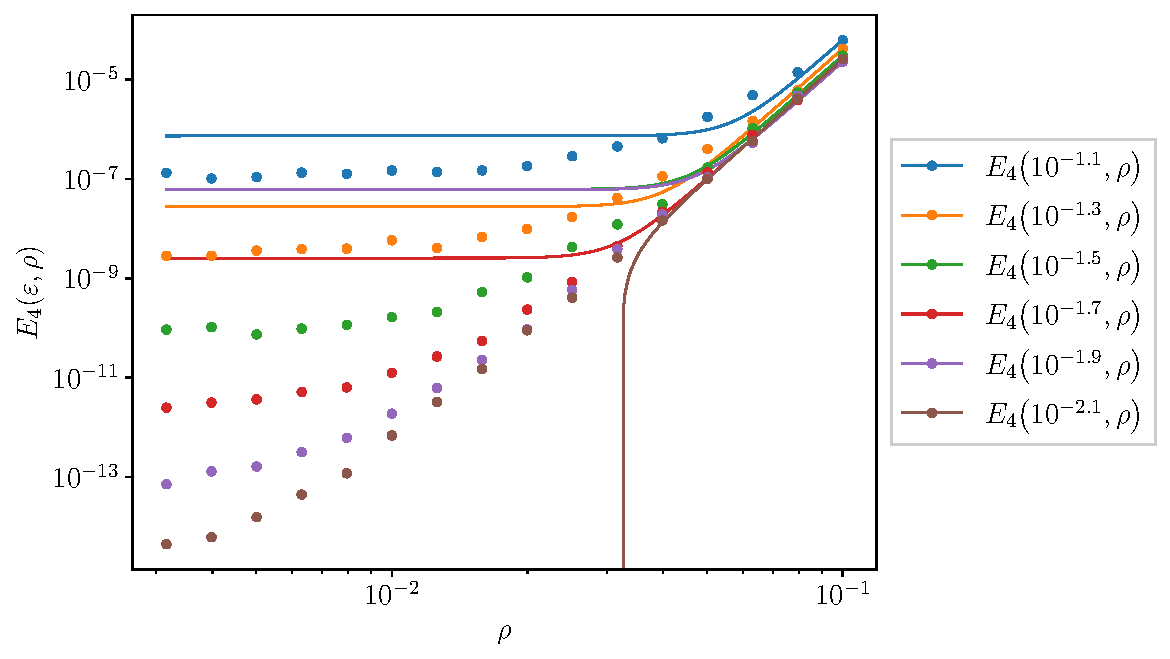
\includegraphics[width=0.49\textwidth]{chp04_paper_numerics/figures/sine/str_err_rho_r_4.0_log.pdf}
% 			\caption{\(r = 4\)}
% 		\end{subfigure}
% 		\caption{}
% 		\label{fig:sine_lines_extra}
% 	\end{center}
% \end{figure}


% \begin{figure}
% 	\begin{center}
% 		\begin{subfigure}{\textwidth}
% 			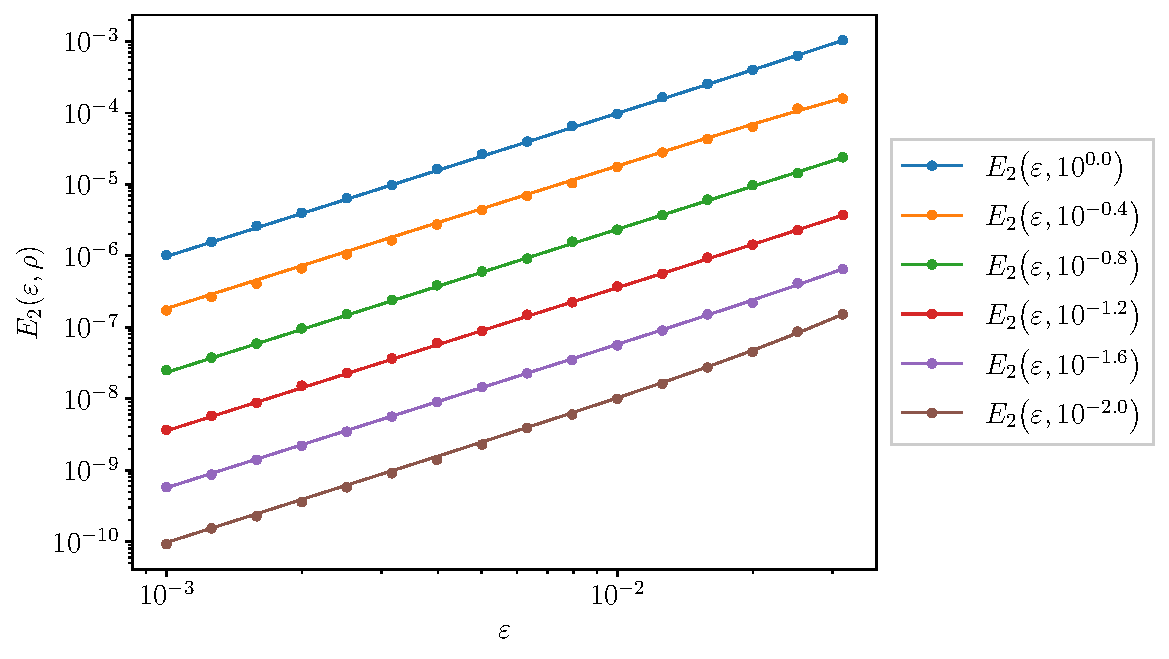
\includegraphics[width=0.49\textwidth]{chp04_paper_numerics/figures/multiplicative/str_err_eps_r_2.0_log.pdf}
% 			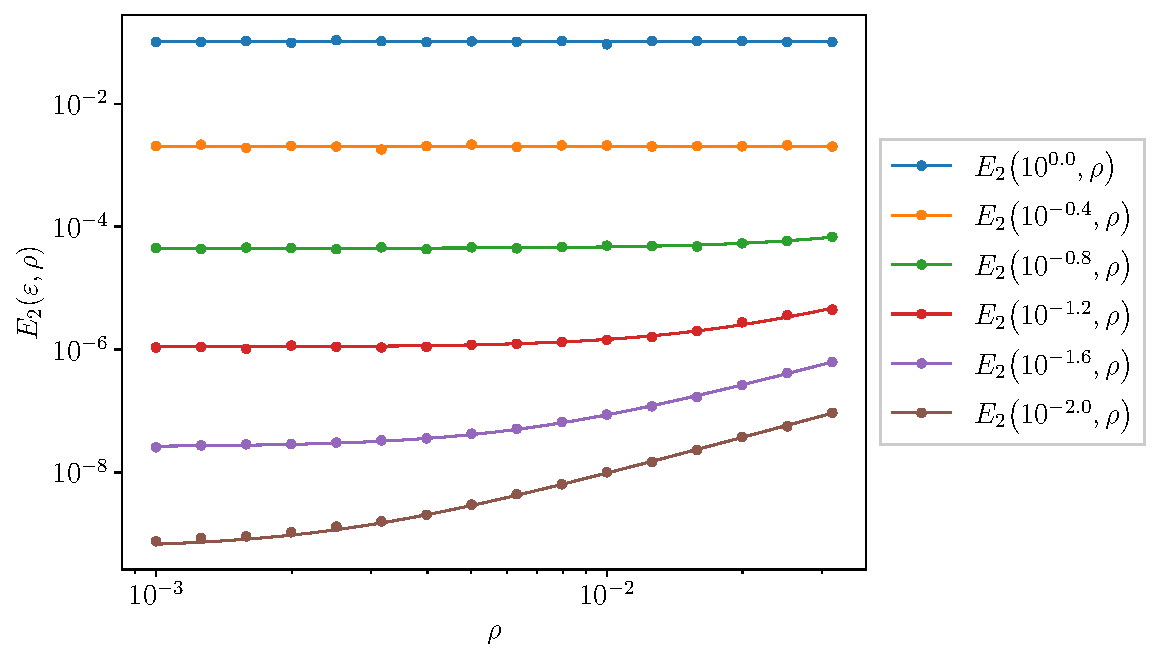
\includegraphics[width=0.49\textwidth]{chp04_paper_numerics/figures/multiplicative/str_err_rho_r_2.0_log.pdf}
% 			\caption{\(r = 2\)}
% 		\end{subfigure}
% 		\begin{subfigure}{\textwidth}
% 			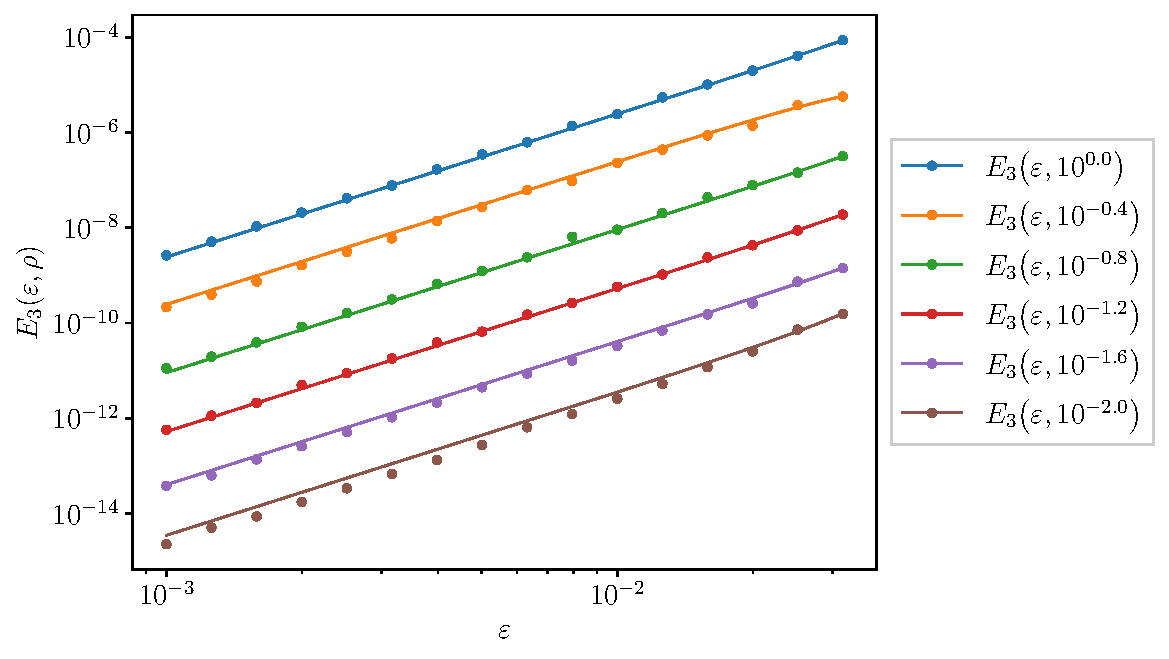
\includegraphics[width=0.49\textwidth]{chp04_paper_numerics/figures/multiplicative/str_err_eps_r_3.0_log.pdf}
% 			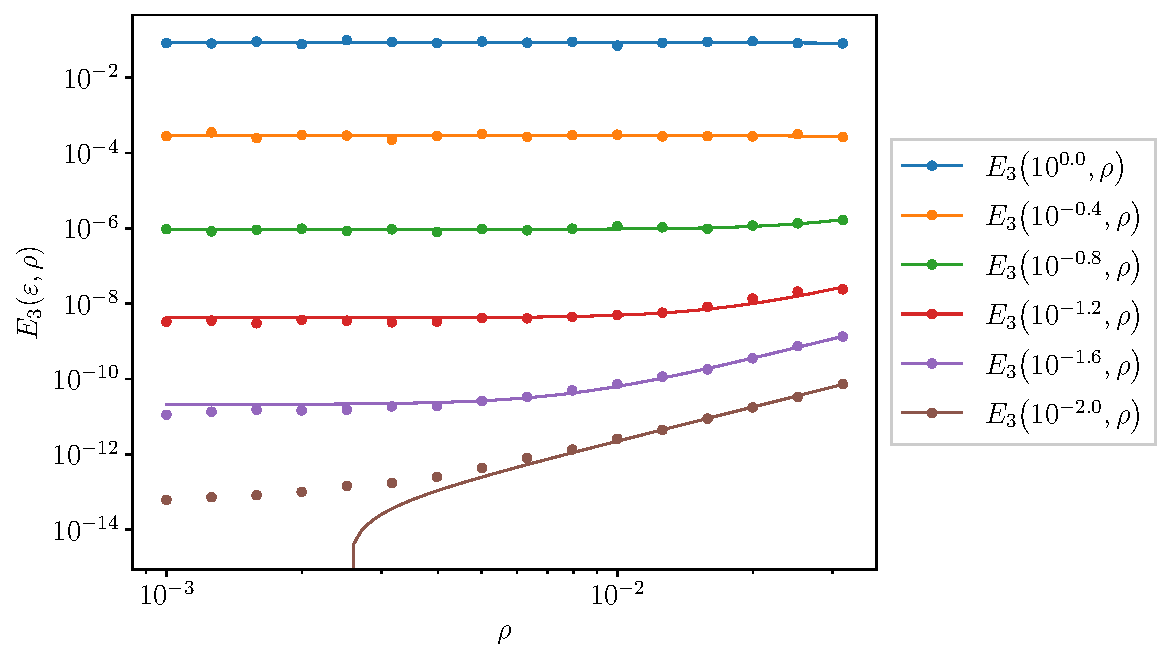
\includegraphics[width=0.49\textwidth]{chp04_paper_numerics/figures/multiplicative/str_err_rho_r_3.0_log.pdf}
% 			\caption{\(r = 3\)}
% 		\end{subfigure}
% 		\begin{subfigure}{\textwidth}
% 			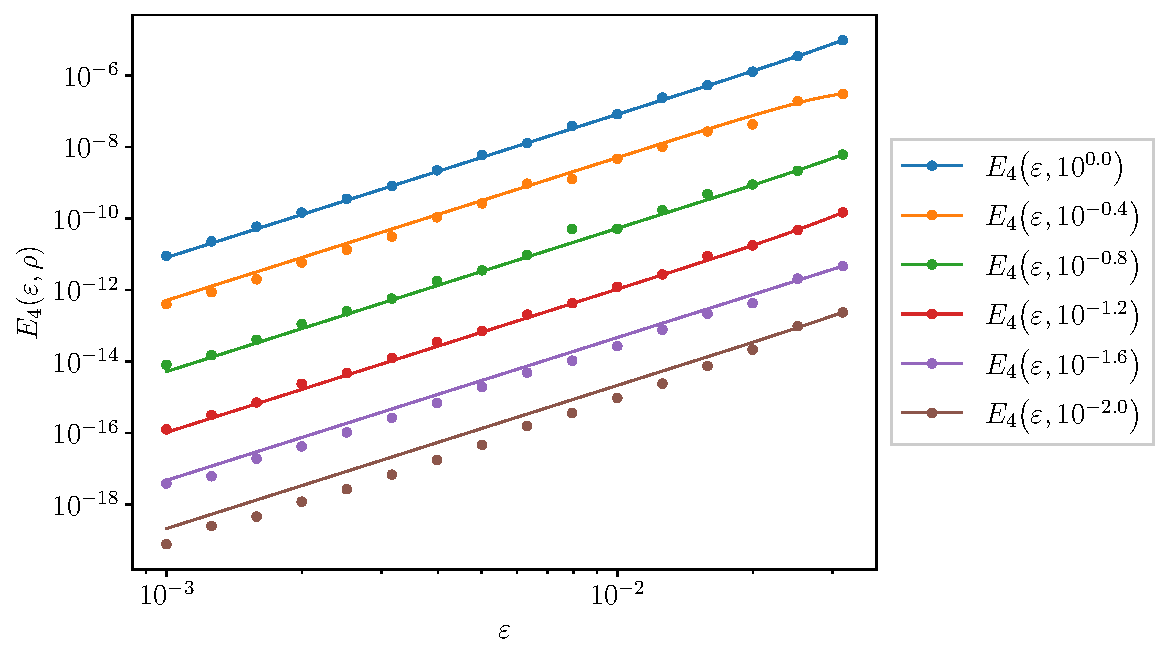
\includegraphics[width=0.49\textwidth]{chp04_paper_numerics/figures/multiplicative/str_err_eps_r_4.0_log.pdf}
% 			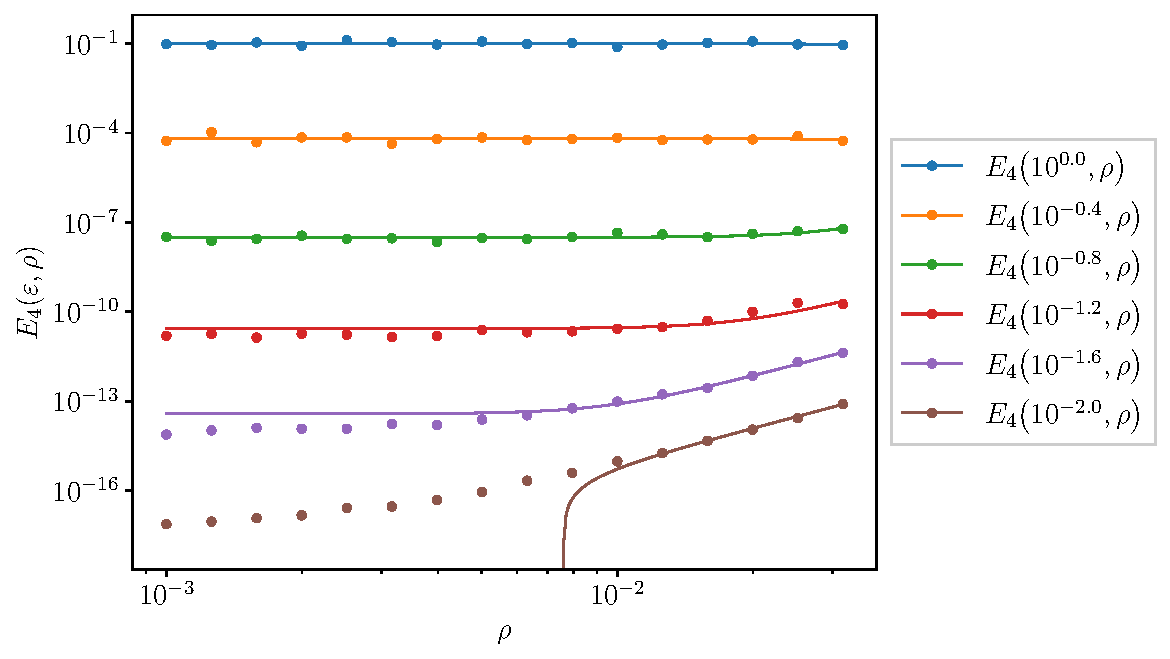
\includegraphics[width=0.49\textwidth]{chp04_paper_numerics/figures/multiplicative/str_err_rho_r_4.0_log.pdf}
% 			\caption{\(r = 4\)}
% 		\end{subfigure}
% 		\caption{}
% 		\label{fig:multiplicative_lines_extra}
% 	\end{center}
% \end{figure}


% % \section{Hellinger distance along Gulf Stream trajectory}\label{app:supp_hell_natl}

% % \begin{figure}
% % 	\begin{center}
% % 		\begin{subfigure}{0.49\textwidth}
% % 			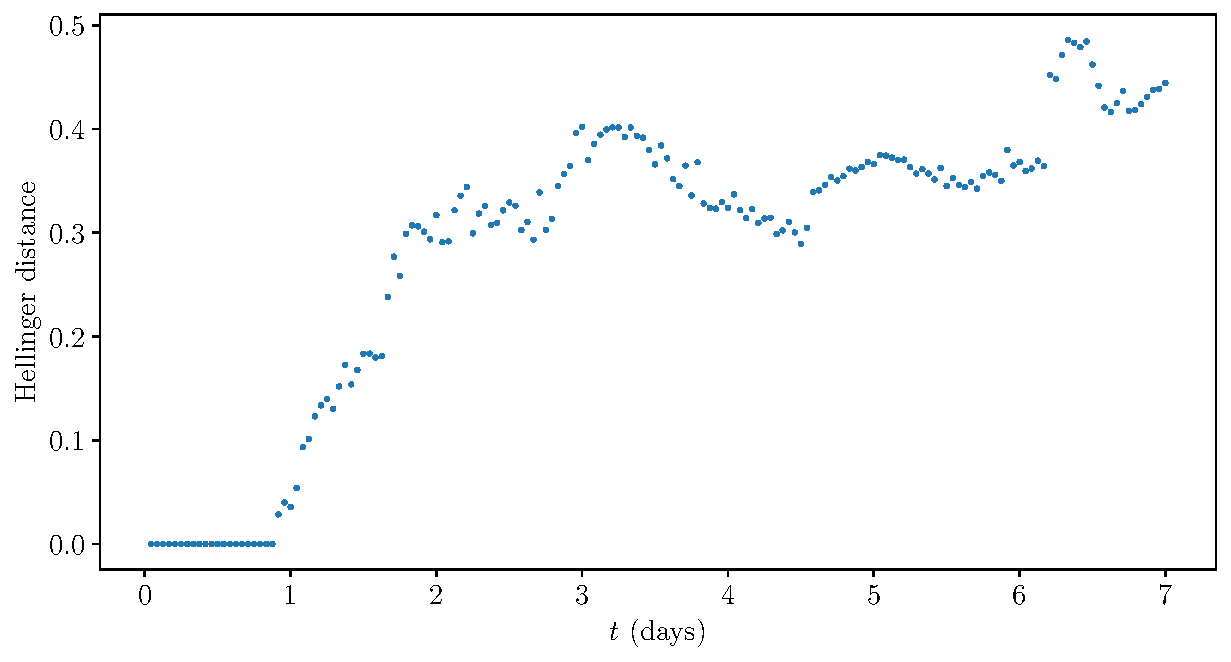
\includegraphics[width=\textwidth]{chp06_applications/figures/gulf_stream/traj_stoch_hell_dist_1.0}
% % 			\caption{\(1^\circ \times 1^\circ\).}
% % 		\end{subfigure}
% % 		\begin{subfigure}{0.49\textwidth}
% % 			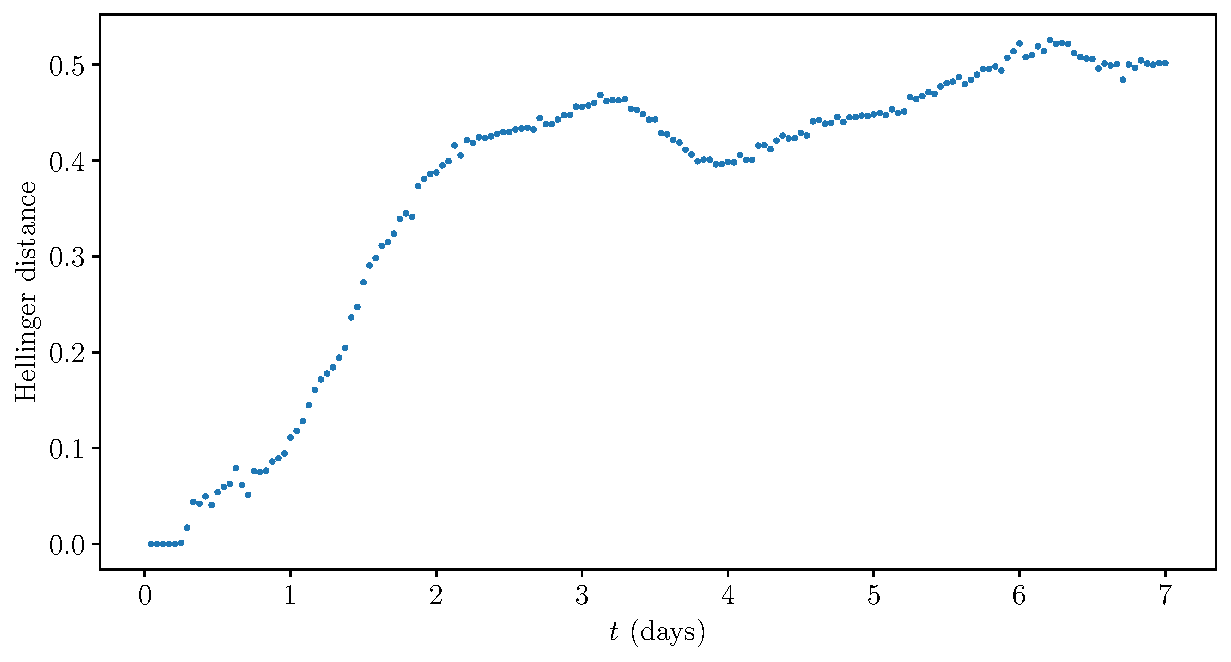
\includegraphics[width=\textwidth]{chp06_applications/figures/gulf_stream/traj_stoch_hell_dist_0.5}
% % 			\caption{\(0.5^\circ \times 0.5^\circ\).}
% % 		\end{subfigure}
% % 		\begin{subfigure}{0.49\textwidth}
% % 			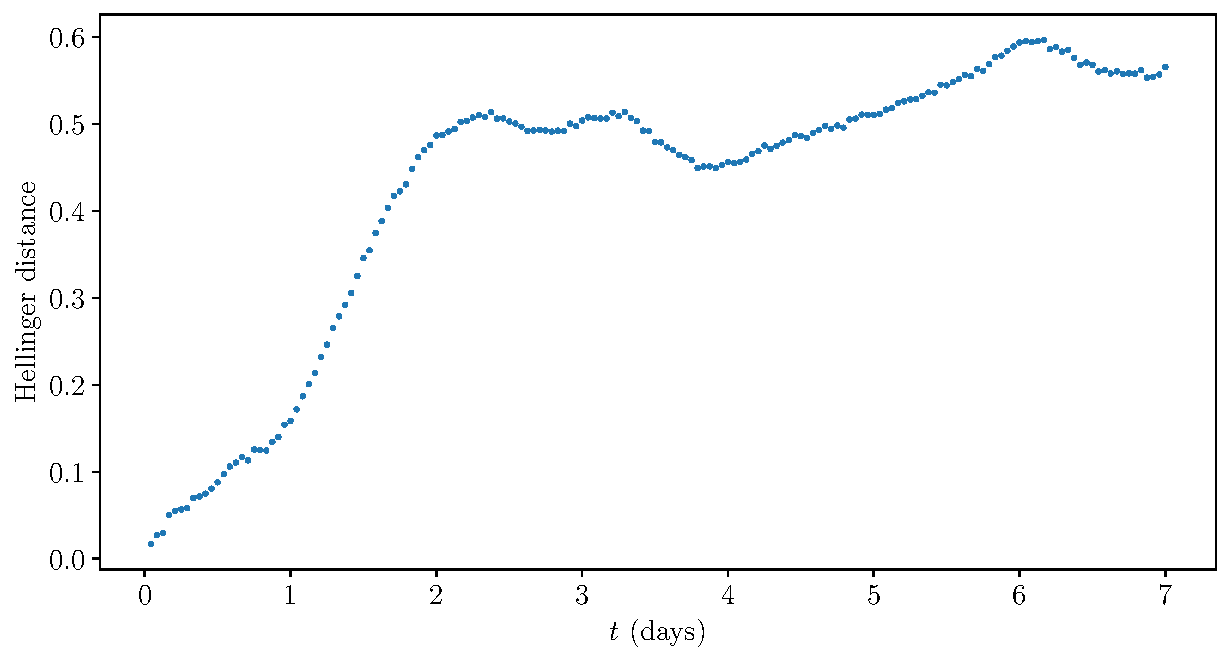
\includegraphics[width=\textwidth]{chp06_applications/figures/gulf_stream/traj_stoch_hell_dist_0.125}
% % 			\caption{\(0.125^\circ \times 0.125^\circ\).}
% % 		\end{subfigure}
% % 		\begin{subfigure}{0.49\textwidth}
% % 			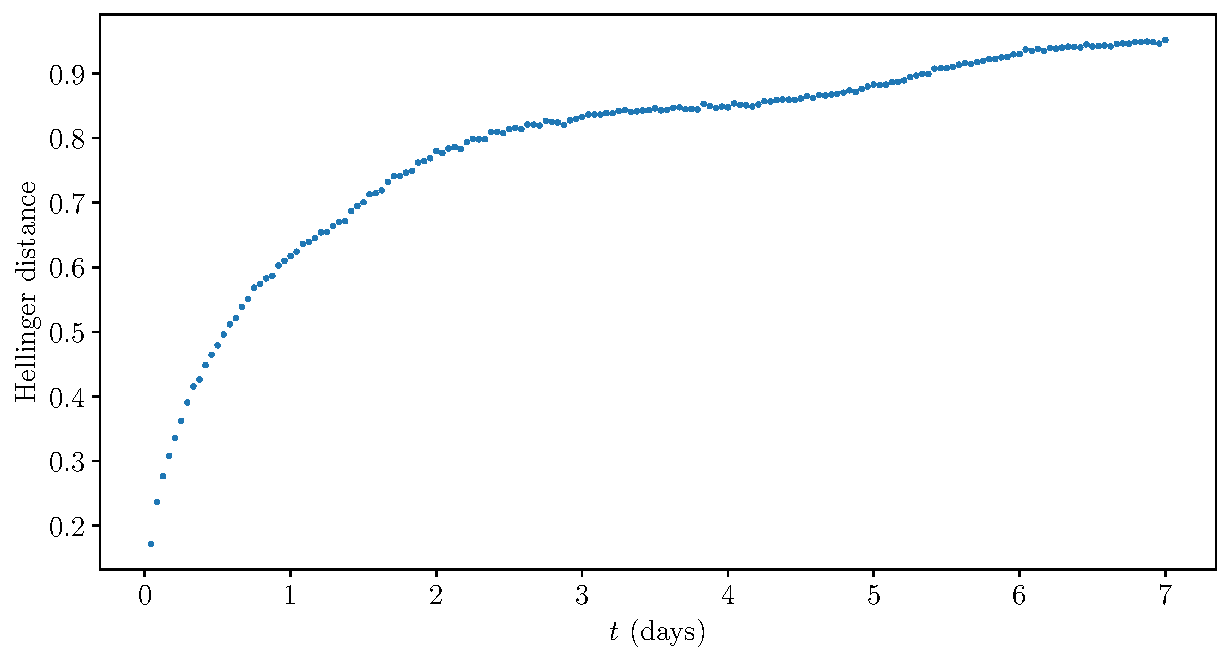
\includegraphics[width=\textwidth]{chp06_applications/figures/gulf_stream/traj_stoch_hell_dist_0.01}
% % 			\caption{\(0.01^\circ \times 0.01^\circ\).}
% % 		\end{subfigure}
% % 		\caption{}
% % 		\label{fig:natl_hell_bwidth}
% % 	\end{center}
% % \end{figure}




\section{Gulf Stream robust sets}\label{app:s2_robust}


\begin{figure}
	\centering
	\begin{subfigure}{\textwidth}
		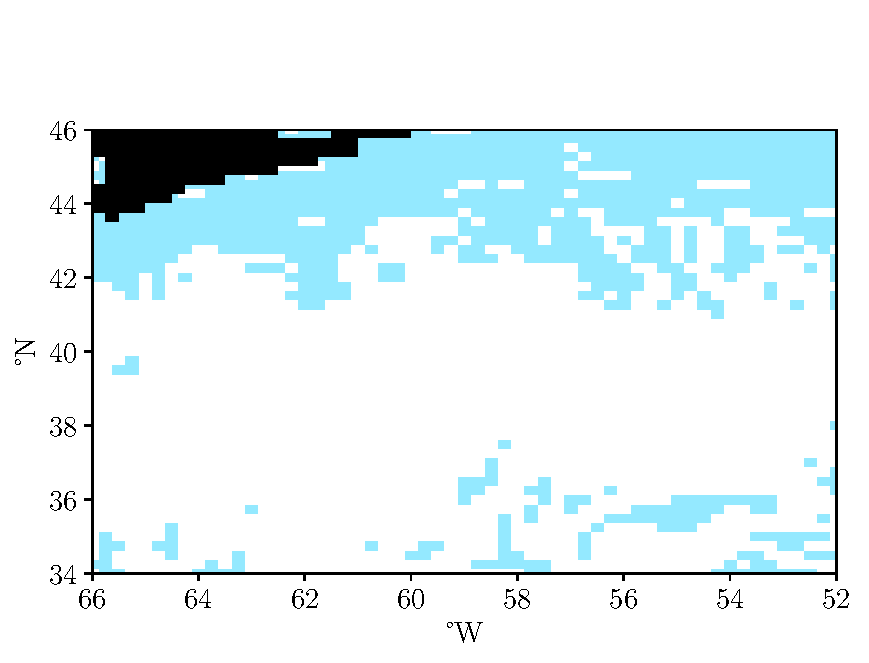
\includegraphics[width=0.5\textwidth]{chp06_applications/figures/gulf_stream/S2_robust_grid_0.25}
		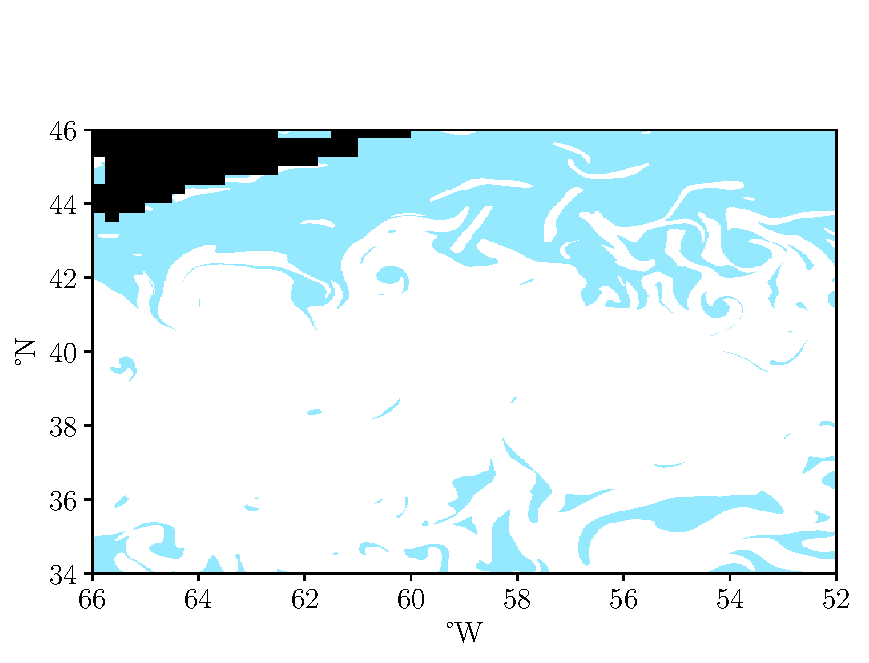
\includegraphics[width=0.5\textwidth]{chp06_applications/figures/gulf_stream/S2_robust_high_0.25}
		\caption{\(R = 0.25^\circ\)}
	\end{subfigure}
	\begin{subfigure}{\textwidth}
		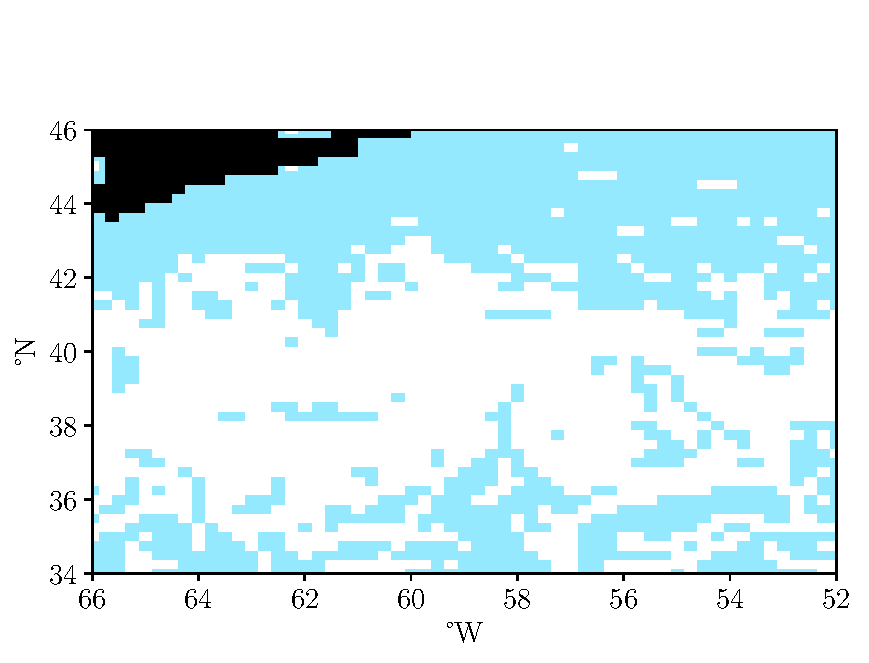
\includegraphics[width=0.5\textwidth]{chp06_applications/figures/gulf_stream/S2_robust_grid_0.5}
		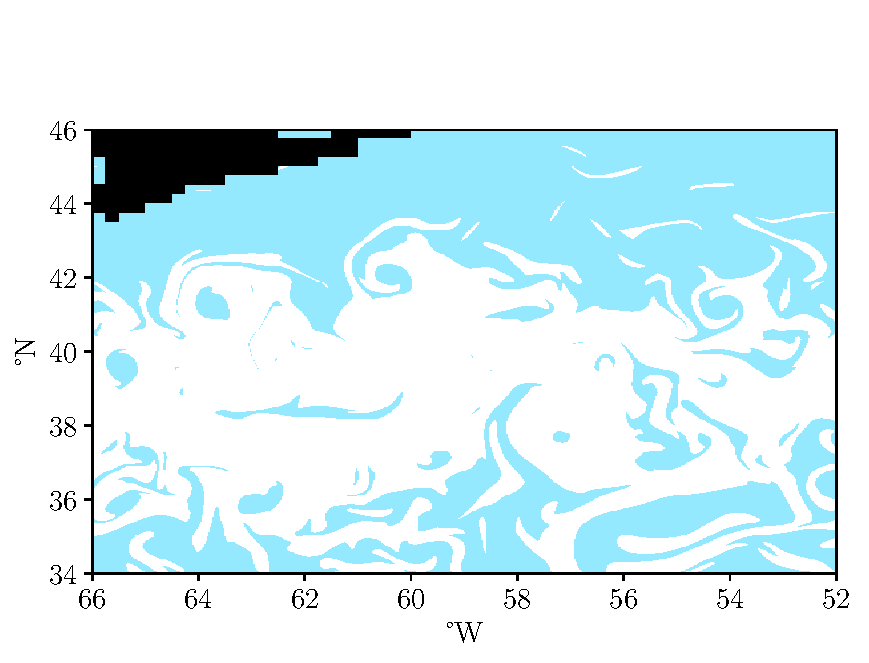
\includegraphics[width=0.5\textwidth]{chp06_applications/figures/gulf_stream/S2_robust_high_0.5}
		\caption{\(R = 0.5^\circ\)}
	\end{subfigure}
	\begin{subfigure}{\textwidth}
		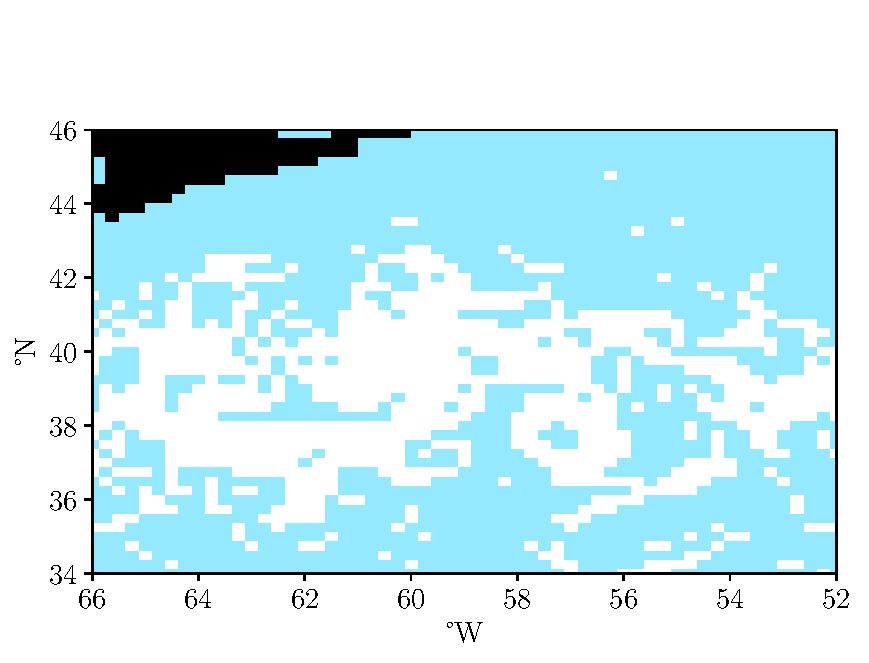
\includegraphics[width=0.5\textwidth]{chp06_applications/figures/gulf_stream/S2_robust_grid_1.0}
		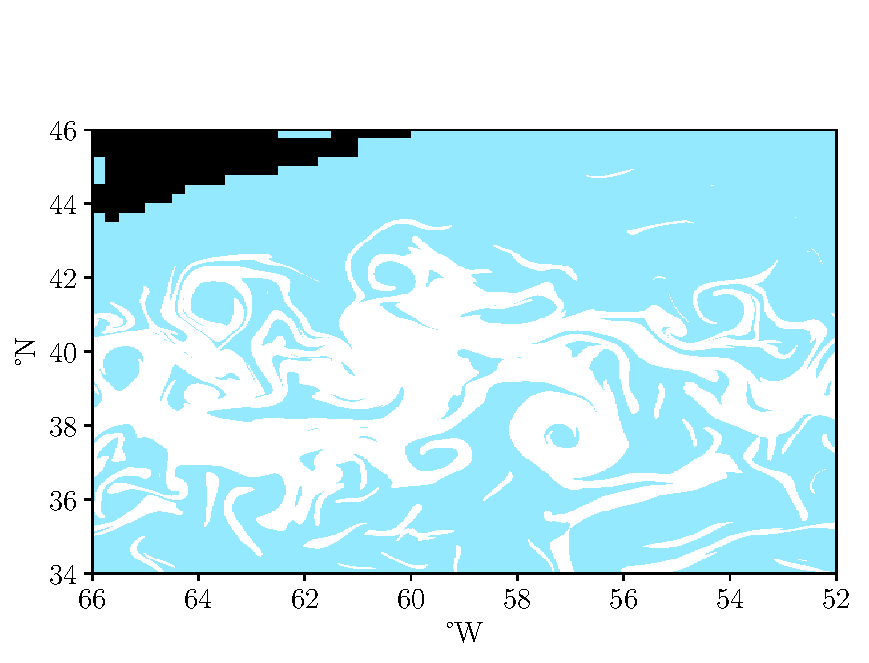
\includegraphics[width=0.5\textwidth]{chp06_applications/figures/gulf_stream/S2_robust_high_1.0}
		\caption{\(R = 1^\circ\)}
	\end{subfigure}
	\begin{subfigure}{\textwidth}
		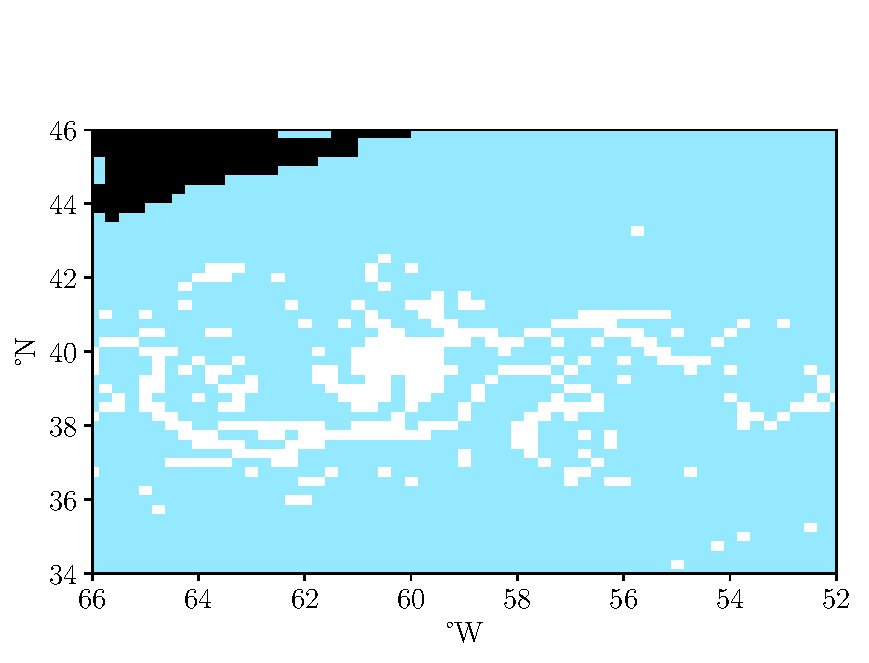
\includegraphics[width=0.5\textwidth]{chp06_applications/figures/gulf_stream/S2_robust_grid_4.0}
		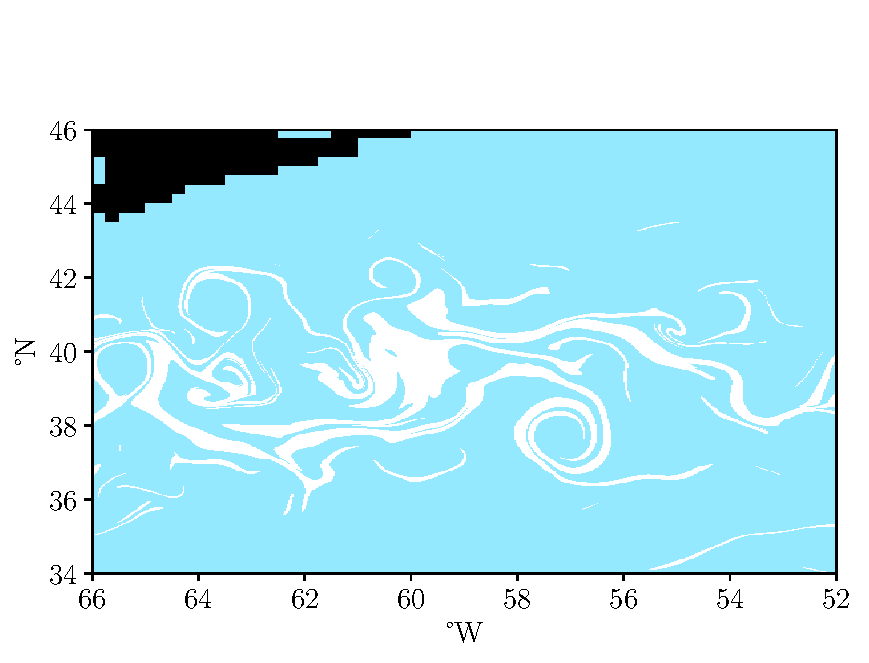
\includegraphics[width=0.5\textwidth]{chp06_applications/figures/gulf_stream/S2_robust_high_4.0}
		\caption{\(R = 4^\circ\)}
	\end{subfigure}
	\begin{subfigure}{\textwidth}
		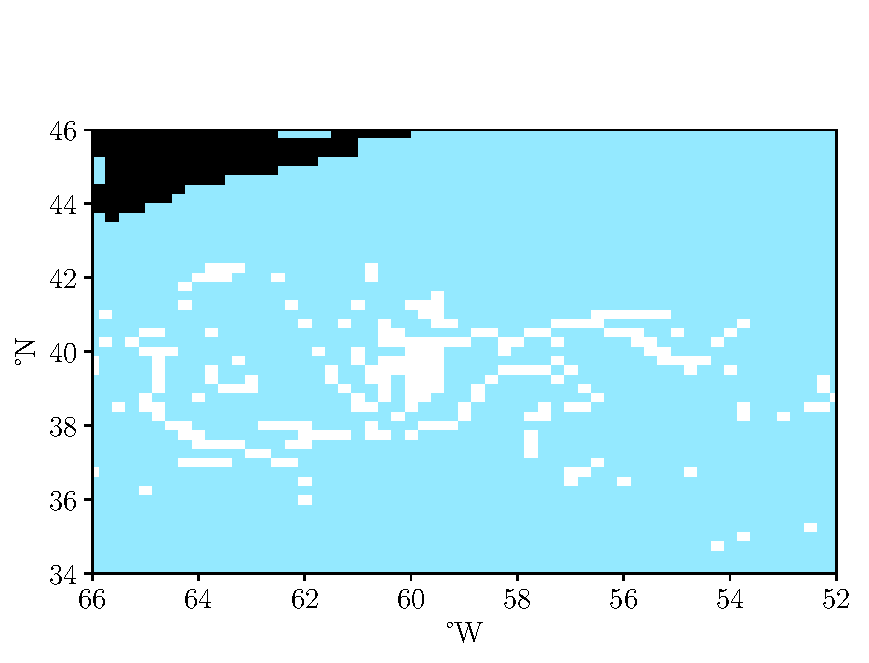
\includegraphics[width=0.5\textwidth]{chp06_applications/figures/gulf_stream/S2_robust_grid_6.0}
		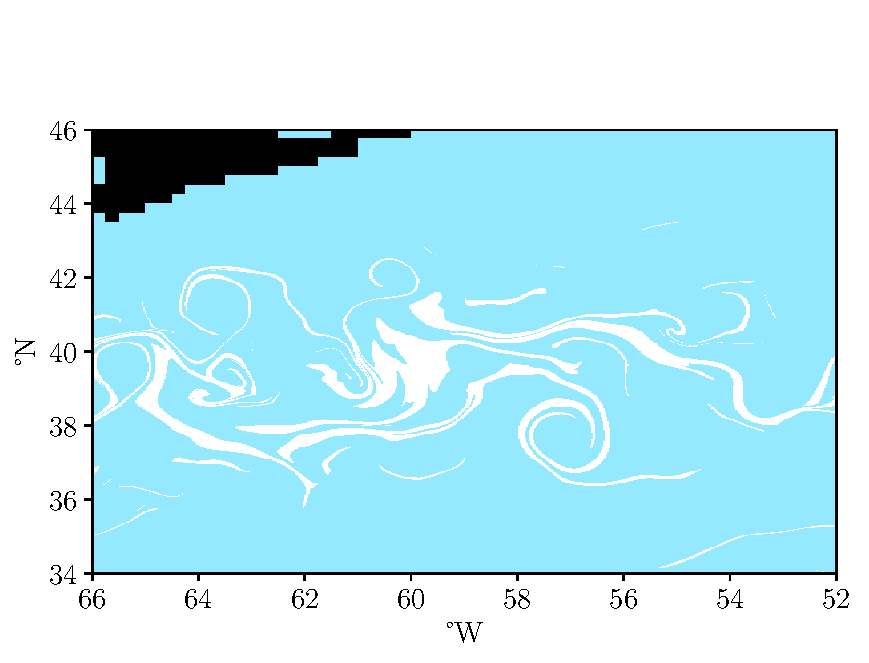
\includegraphics[width=0.5\textwidth]{chp06_applications/figures/gulf_stream/S2_robust_high_6.0}
		\caption{\(R = 6^\circ\)}
	\end{subfigure}
	\caption{Robust sets extracted from the stochastic sensitivity field using different thresholds \(R\) on the Gulf Stream example, at the resolution of the data (left) and the increased resolution \(0.025^\circ \times 0.025^\circ\).}
	\label{fig:na_robust_extra}
\end{figure}
